\documentclass[8pt]{beamer}
\usepackage[polish]{babel}
\usepackage[utf8]{inputenc}
\usepackage[T4]{fontenc}
\usepackage{subcaption}
\usepackage{multicol}
%\usepackage{pgfpages}



\title[Robotyczne protezy ręki, BeBionic]{Sprzężenie zwrotne w robotycznych protezach ręki}

\date[2013]{13.12.2013}
\author[inż. Paweł Bogner, inż. Grzegorz Maj]{inż. Paweł Bogner, inż. Grzegorz Maj}
\institute[PWr]{Politechnika Wrocławska}

\setbeamercovered{transparent=10}
\usetheme{Warsaw}
\bibliographystyle{plain}

\begin{document}
{
\frame{\maketitle}
}

\begin{frame}{Plan}
%	\begin{itemize}
%		\item Przegląd dostępnych protez.
%		\item Budowa robotycznych rąk.
%		\item Ręka Bebionic.
%		\item Sprzężenie zwrotne.
%		\item Propozycja rozwinięcia ręki BeBionic.
%	\end{itemize}
\begin{multicols}{2}
	\tableofcontents
	\end{multicols}
\end{frame}

\section{Przegląd dostępnych protez}

\begin{frame}%{Przegląd dostępnych protez}
	\begin{center}
		\begin{figure}
			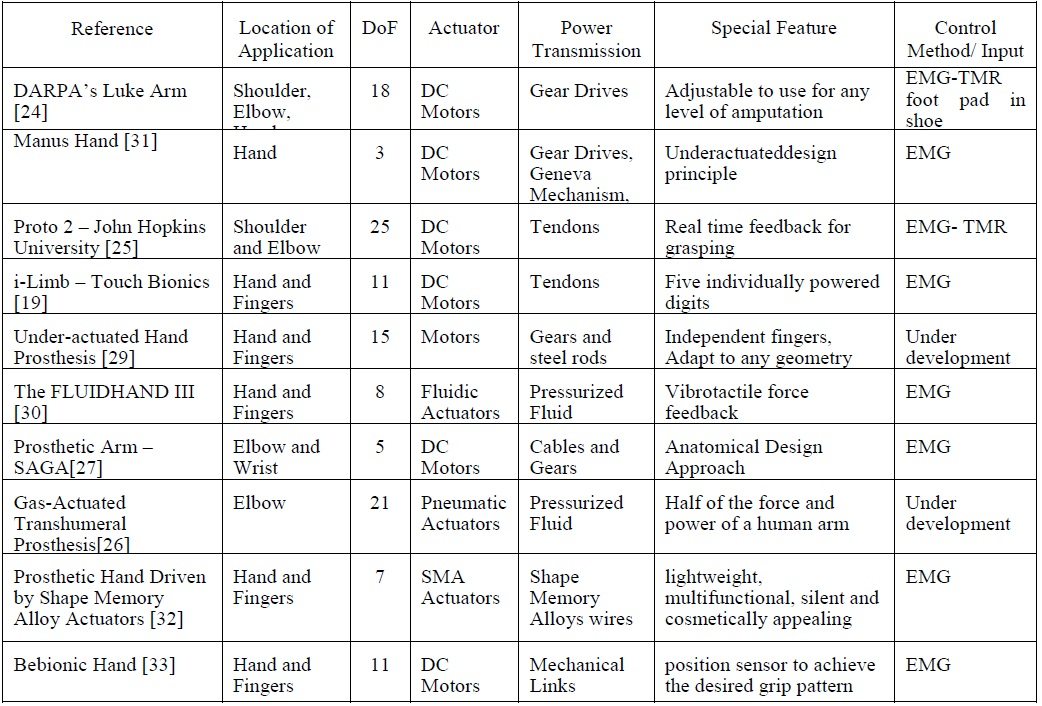
\includegraphics[width=0.7\textwidth]{graphics/hands.jpg}
			\label{graph:hand}	
			\caption{Przegląd rąk \cite{bandara2012upper}}
		\end{figure}
	\end{center}

\end{frame}

\begin{frame}%{Przegląd dostępnych protez}
	\begin{center}
		\begin{figure}
			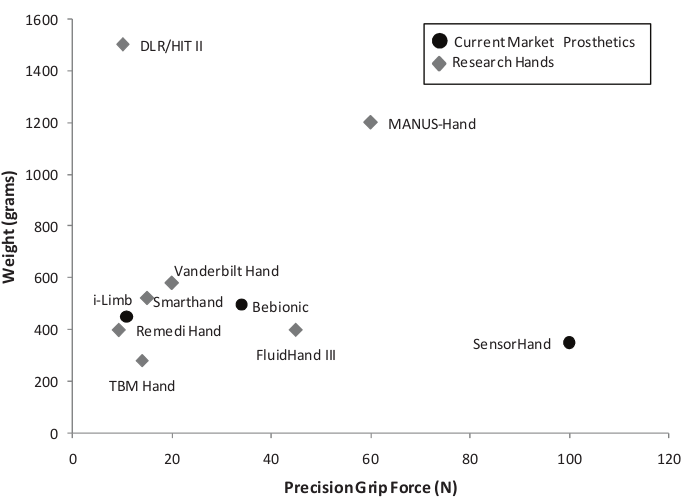
\includegraphics[width=0.7\textwidth]{graphics/weight_gripforce.png}
			\label{graph:hand}	
			\caption{Porównanie dostępnych protez \cite{belter2011performance}.}
		\end{figure}
	\end{center}

\end{frame}
 
\begin{frame}%{Przegląd dostępnych protez}
	\begin{center}
		\begin{figure}
			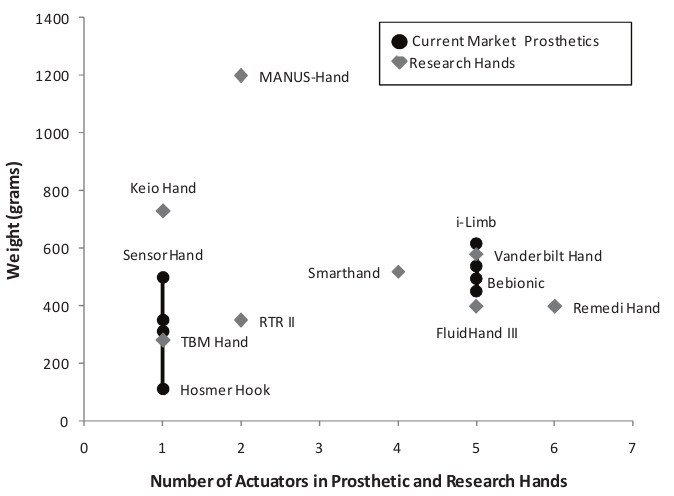
\includegraphics[width=0.7\textwidth]{graphics/weight_actuators.png}
			\label{graph:hand}	
			\caption{Porównanie dostępnych protez \cite{belter2011performance}.}
		\end{figure}
	\end{center}

\end{frame}

\begin{frame}%{Przegląd dostępnych protez}
	\begin{center}
		\begin{figure}
			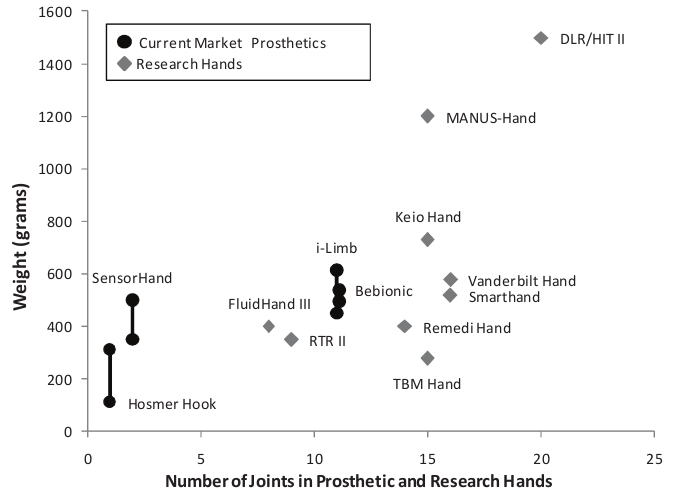
\includegraphics[width=0.7\textwidth]{graphics/weight_joints.png}
			\label{graph:hand}	
			\caption{Porównanie dostępnych protez \cite{belter2011performance}.}
		\end{figure}
	\end{center}

\end{frame}

\begin{frame}%{Przegląd dostępnych protez}
	\begin{center}
		\begin{figure}
			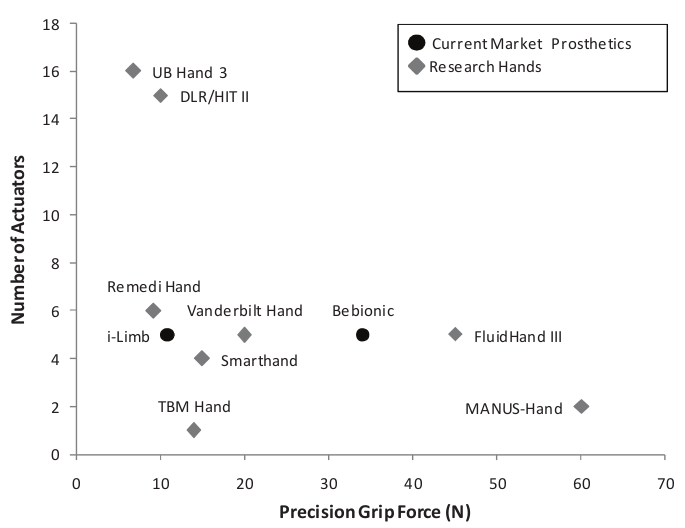
\includegraphics[width=0.7\textwidth]{graphics/actuators_gripforce.png}
			\label{graph:hand}	
			\caption{Porównanie dostępnych protez \cite{belter2011performance}.}
		\end{figure}
	\end{center}

\end{frame}

\begin{frame}%{Przegląd dostępnych protez}
	\begin{center}
		\begin{figure}
			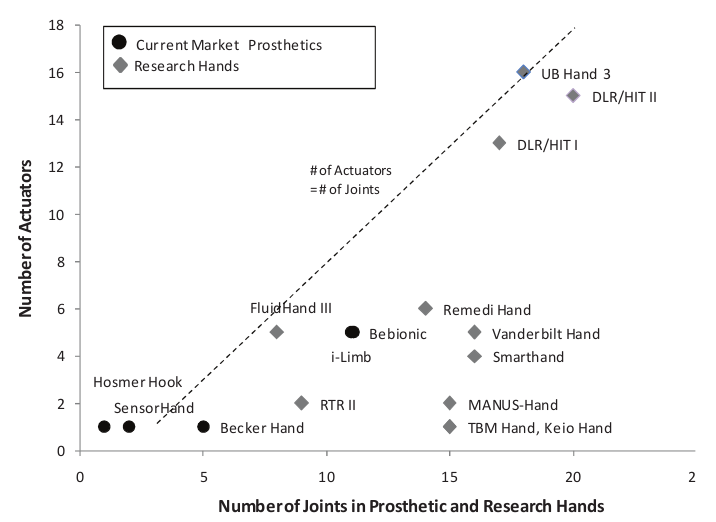
\includegraphics[width=0.7\textwidth]{graphics/actuators_joints.png}
			\label{graph:hand}	
			\caption{Porównanie dostępnych protez \cite{belter2011performance}.}
		\end{figure}
	\end{center}

\end{frame}


	\subsection{Podział}
		\begin{frame}
			\begin{center}
				\begin{figure}
					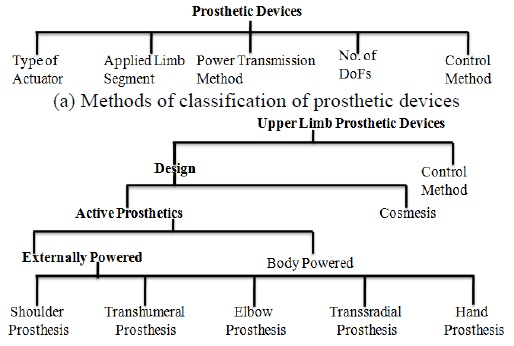
\includegraphics[width=0.7\textwidth]{graphics/classification.jpg}
					\label{graph:class}	
					\caption{Klasyfikacja \cite{bandara2012upper}}
				\end{figure}
			\end{center}
		\end{frame}							

\section{Budowa robotycznych rąk}

	\subsection{Budowa dłoni}
		\begin{frame}
			\begin{center}
				\begin{figure}
					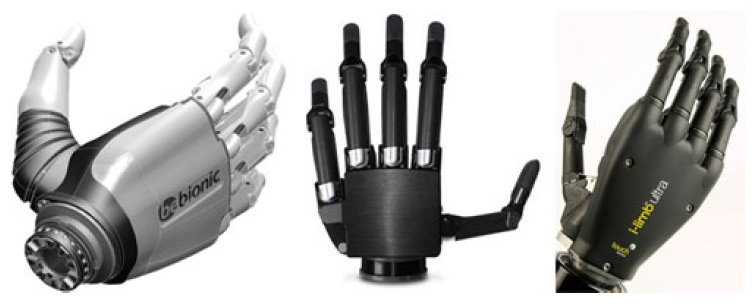
\includegraphics[width=\textwidth]{graphics/three_hand.jpg}
					\label{graph:build}	
					\caption{ \cite{6361492}}
				\end{figure}
			\end{center}
		\end{frame}				

	\subsection{Sterowanie palcem}
		\begin{frame}
			\begin{center}
				\begin{figure}
					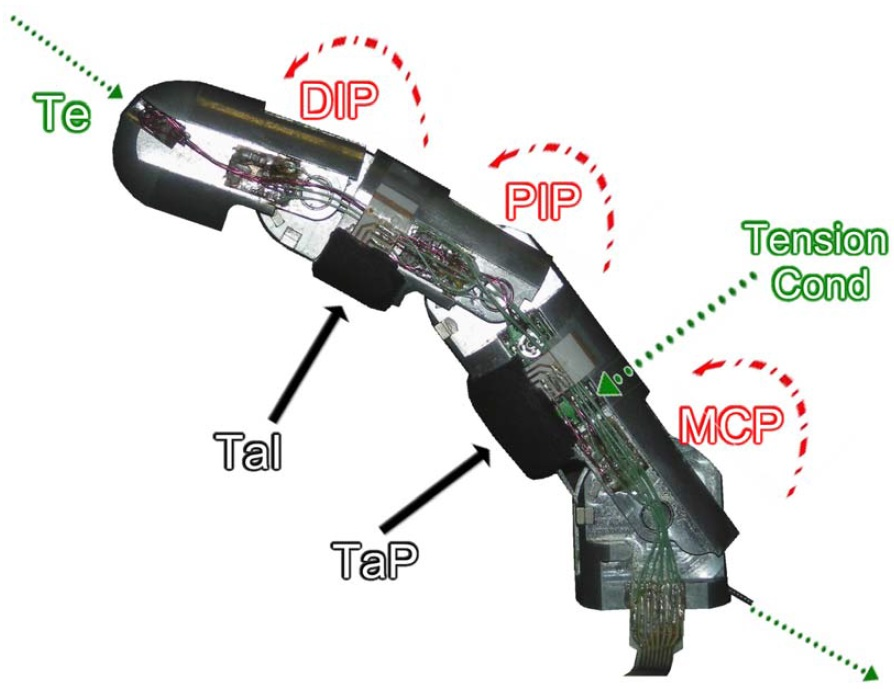
\includegraphics[width=0.7\textwidth]{graphics/smarthand_finger.jpg}
					\label{graph:build}	
					\caption{ \cite{6361492}}
				\end{figure}
			\end{center}
		\end{frame}				

		\begin{frame}
			\begin{center}
				\begin{figure}
					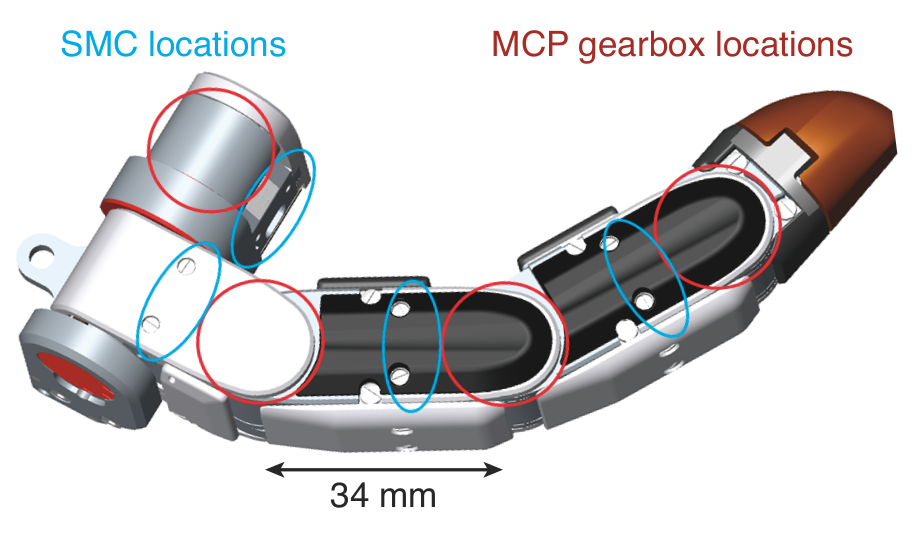
\includegraphics[width=0.7\textwidth]{graphics/finger_motors_mpl.png}
					\label{graph:build}	
					\caption{ \cite{6361492}}
				\end{figure}
			\end{center}
		\end{frame}				


	\subsection{Rodzaje chwytów}
		\begin{frame}[allowframebreaks]
			\begin{center}
				\begin{figure}
				\centering
				\begin{subfigure}[b]{0.4\textwidth}
                		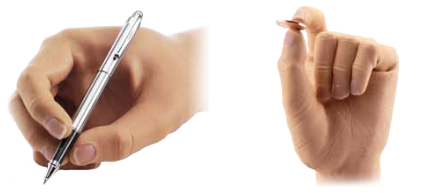
\includegraphics[width=\textwidth]{graphics/grip1.png}
                		\caption{Chwyt: trójpunktowy, dwupunktowy.}
                		\label{graph:g1}
        			\end{subfigure}%
        			\begin{subfigure}[b]{0.4\textwidth}
                		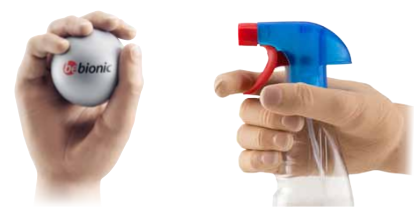
\includegraphics[width=\textwidth]{graphics/grip2.png}
                		\caption{Chwyt: siłowy, aktywny wskaziciel.}
                		\label{graph:g2}
        			\end{subfigure}%
        			\newline
        			\begin{subfigure}[b]{0.4\textwidth}
                		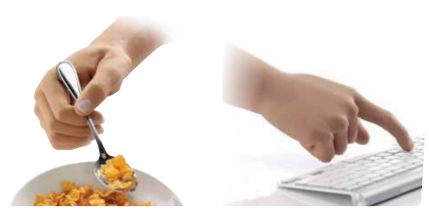
\includegraphics[width=\textwidth]{graphics/grip3.png}
                		\caption{Chwyt: boczny, wskazywanie.}
                		\label{graph:g3}
        			\end{subfigure}%
        			\begin{subfigure}[b]{0.4\textwidth}
                		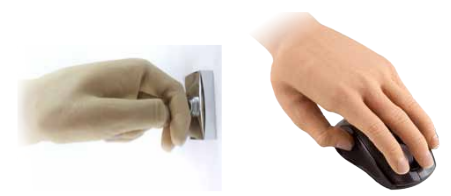
\includegraphics[width=\textwidth]{graphics/grip4.png}
                		\caption{Chwyt: kolumnowy, do myszki.}
                		\label{graph:g4}
        			\end{subfigure}%
				\newline
        			\begin{subfigure}[b]{0.4\textwidth}
                		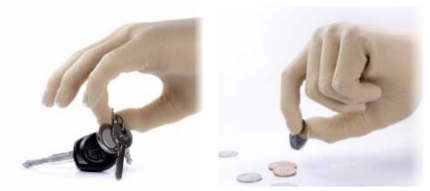
\includegraphics[width=\textwidth]{graphics/grip5.png}
                		\caption{Chwyt: precyzyjny.}
                		\label{graph:g5}
        			\end{subfigure}%
        			\begin{subfigure}[b]{0.4\textwidth}
                		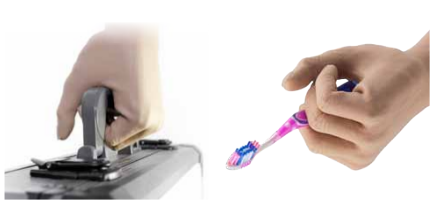
\includegraphics[width=\textwidth]{graphics/grip6.png}
                		\caption{Chwyt: hakowy, koncentryczny.}
                		\label{graph:g6}
        			\end{subfigure}%
        			\newline
        			\begin{subfigure}[b]{0.4\textwidth}
                		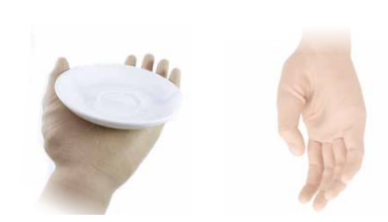
\includegraphics[width=\textwidth]{graphics/grip7.png}
                		\caption{Chwyt: otwarta dłoń, luźna ręka}
                		\label{graph:g7}
        			\end{subfigure}%
        			\end{figure}
				\end{center}
			
		\end{frame}
%				\end{figure}
%			\end{center}
%		\end{frame}				
%		
%		\begin{frame}
%			\begin{figure}
%				\begin{center}1

\section{Ręka Bebionic}

	\begin{frame}%{Ręka Bebionic}
		bebionic3
		\begin{itemize}[<+->]
	\item osobne silniki na każdy palec, rozmieszczenie optymalnosiłowe,
	\item wydajne mikroprocesory ciągle monitorują pozycję każdego palca, dając pełną kontrolę nad protezą.
	\item 14 różnych rodzajów chwytów,
	\item adekwatna kontrola prędkości pozwala na wykonywanie precyzyjnych ruchów,
	\item możliwość przestawienia pozycji kciuka na pozycję przeciwstawną (ręczne),
	\item automatyczna kontrola siły uścisku zapobiega wyślizgiwaniu się przedmiotów,
	\item palce uginają się naturalnie przy zderzaniu się z obiektami,
	\item możliwość noszenia przedmiotów o masie do 45 kg,
		\end{itemize}

	\end{frame}

	\subsection{Podstawowa budowa}
	\begin{frame}
	\begin{center}
				\begin{figure}
					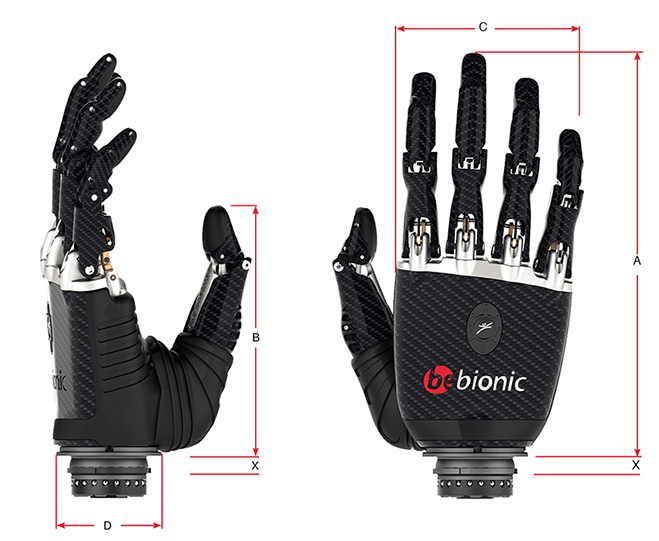
\includegraphics[width=0.7\textwidth]{graphics/bebionic_dimentions.jpg}
					\label{graph:grasp}	
					\caption{ \cite{bebionic}}
				\end{figure}
			\end{center}
	\end{frame}		
	
		\begin{frame}
		\frametitle{Specyfikacja dłoni}

		\begin{itemize}
\item A Middle Finger Tip to Hand Base	 200mm	 190mm\\
\item B Thumb Tip to Hand Base	 125mm	 121mm\\
\item C Max Chassis Width (no glove)	 92mm	 84mm\\
\item D Diameter of Chassis at Wrist	 50mm	 50mm\\
\item Palm Circumference (no glove)	 220mm	 204mm\\
\item Maximum Opening width Tripod Grip	 105mm with glove	 105mm with glove\\
\item Weight	 557g – 598g	 550g -- 591g\\
\item Maximum Power Grip	 140.1N\\
\item Maximum Tripod Grip	 36.6N\\
\item Maximum Key Grip	 26.5N\\
\item Minimum Time to Open \/ Close -- Tripod Grip	 0.5 Seconds\\
\item Minimum Time to Open \/ Close -- Power Grip	 0.5 Seconds\\
\item Minimum Time to Open \/ Close -- Key Grip	 1.0 Seconds\\
\item Maximum Static Load -- Hook Grip	 45kg\\
\item Maximum Load Individual Finger -- Hook Grip	 25kg\\
		\end{itemize}		
		\end{frame}				

	\subsection{Możliwości dostrajania}
		\begin{frame}
		
		Rękę BeBionic można dostrajać za pomocą oprogramowania dostarczanego  wraz z protezą.
		Program Bebalance umożliwia dostosowanie siły i prędkości uchwytu oraz wybór sposobu ruchu ręki. Wszystko odbywa się bezprzewodowo co daje możliwość nie ściągania protezy podczas jej dostrajania.

		\end{frame}	
		
		\begin{frame}
		\begin{center}
			\begin{figure}
				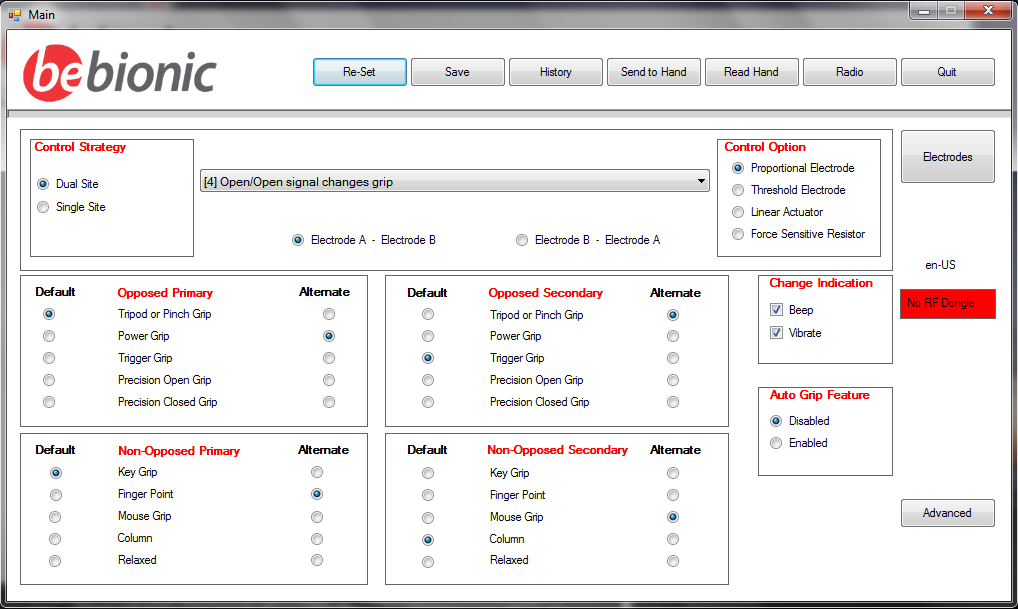
\includegraphics[width=\textwidth]{graphics/bebelance.png}
				\label{graph:feedback}	
			\end{figure}
			\end{center}
		\end{frame}			
		
		\begin{frame}
		\begin{center}
			\begin{figure}
				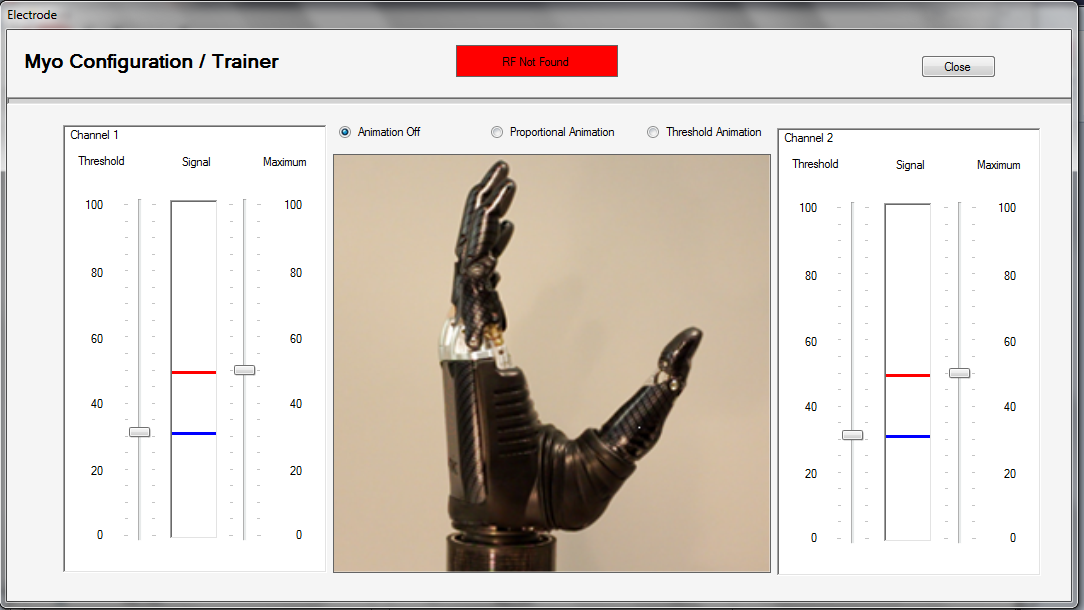
\includegraphics[width=\textwidth]{graphics/bebelance2.png}
				\label{graph:feedback}	
			\end{figure}
			\end{center}
		\end{frame}		

\section{Sprzężenie zwrotne}

\begin{frame}%{Sprzężenie zwrotne}
	\begin{center}
		\begin{figure}
			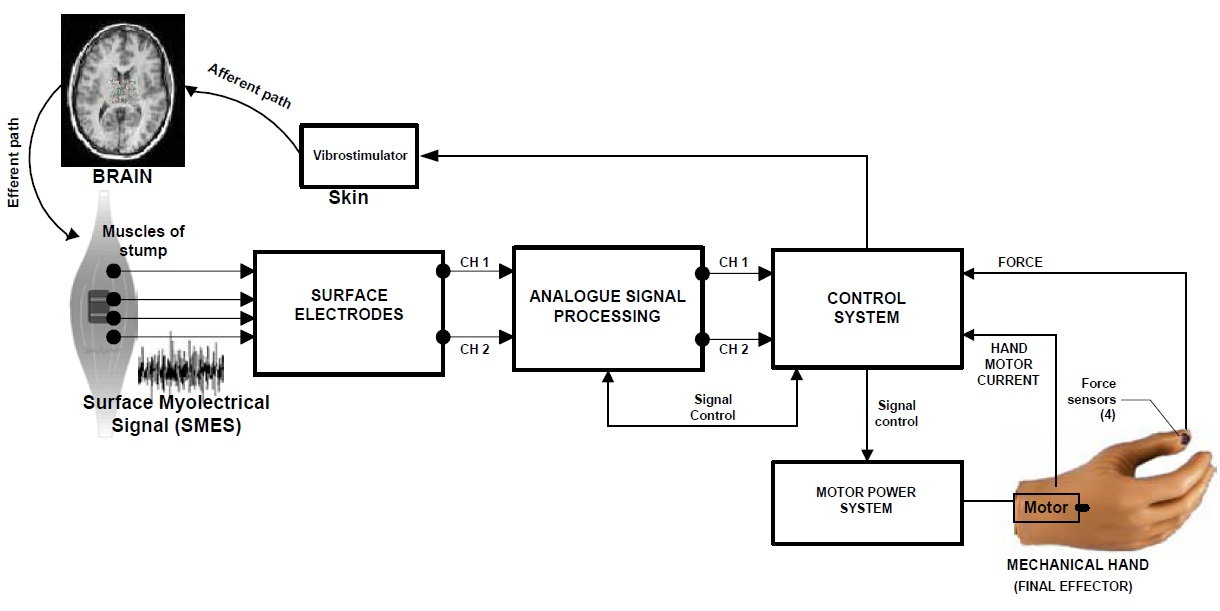
\includegraphics[width=\textwidth]{graphics/feedback.jpg}
			\label{graph:feedback}	
		\end{figure}
	\end{center}
	%\note{omówić cały obrazek}
\end{frame}

	\subsection{Oczekiwania pacjentów}
		\begin{frame}
			\begin{center}
				\begin{figure}
					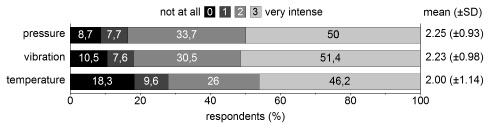
\includegraphics[width=\textwidth]{graphics/sensitivity.jpg}
					\label{graph:feedback2}	
					\caption{Jak mocno doświadczasz następujących odczuć poprzez kikut? \cite{6226669}}
				\end{figure}
			\end{center}
		\end{frame}			
	
						
		
		\begin{frame}
			\begin{center}
				\begin{figure}
					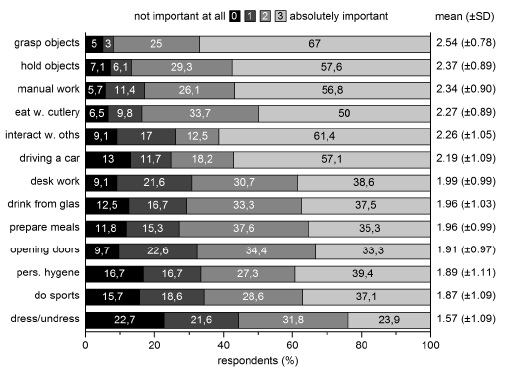
\includegraphics[width=0.8\textwidth]{graphics/activities.jpg}
					\label{graph:feedback2}	
					\caption{Jak ważne jest sprzężenie zwrotne z protezy podczas poszczególnych czynności? \cite{6226669}}
				\end{figure}
			\end{center}
		\end{frame}		
		
		\begin{frame}
			\begin{center}
				\begin{figure}
					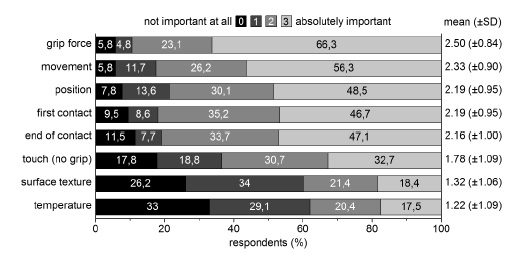
\includegraphics[width=\textwidth]{graphics/sensory_info.jpg}
					\label{graph:feedback2}	
					\caption{Jak ważne są poszczególne odczucia z protezy? \cite{6226669}}
				\end{figure}
			\end{center}
		\end{frame}		
		
		\begin{frame}
			\begin{center}
				\begin{figure}
					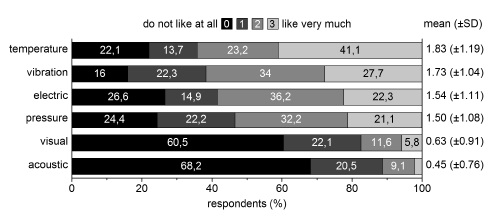
\includegraphics[width=\textwidth]{graphics/way_of_feedback.jpg}
					\label{graph:feedback2}	
					\caption{W jaki sposób chciałbyś odbierać odczucia z protezy?  \cite{6226669}}
				\end{figure}
			\end{center}
		\end{frame}
		
		
		\begin{frame}
		\begin{center}
		\begin{table}
			\begin{tabular}{|c|c|c|c|c|c|}
			\hline
			 & Use of & & & &\\
			Perception & perception & Grasp & Hold & Proprioception & Sum \\
			\hline
			Visual observation & 77\% & 15 & 2 & 18 & 35 \\
			\hline
			Listening & 67\% & 7 & 1 & 14 & 22 \\
			\hline
			Sensations at residual limb & 57\% & 1 & 12 & 1 & 14\\
			\hline
			\end{tabular}								
			\caption{Użycie sprzężenia zwrotnego w dotychczasowych protezach.}
		\end{table}
		\end{center}		
		
		\begin{center}
		\begin{table}
		
			\begin{tabular}{|c|c|c|c|}
			\hline
			 & 1 & 2 & 3 \\
			\hline
			grasp and hold & 59\% & 46\% & 35\% \\
			\hline
			touch & 17\% & 29\% & 32\% \\
			\hline
			proprioception & 22\% & 23\% & 31\% \\
			\hline
			\end{tabular}	
			\caption{Najważniejsze informacje zwrotne z protezy.}						
		\end{table}
		\end{center}
		
		

			
		\end{frame}

	\subsection{Pobieranie informacji}
		\begin{frame}
		Potrzebne sygnały:
			\begin{itemize}[<+->]
				\item siła uchwytu,
				\item ruch,
				\item pozycja,
				\item początek kontaktu,
				\item koniec kontaktu,
				\item dotyk, 
				\item struktura powierzchni,
				\item temperatura.
			\end{itemize}
		\end{frame}		
		
		
		
		\subsection{Przekazanie informacji od/do pacjenta}	
		\begin{frame}
			\begin{center}
				\begin{figure}
					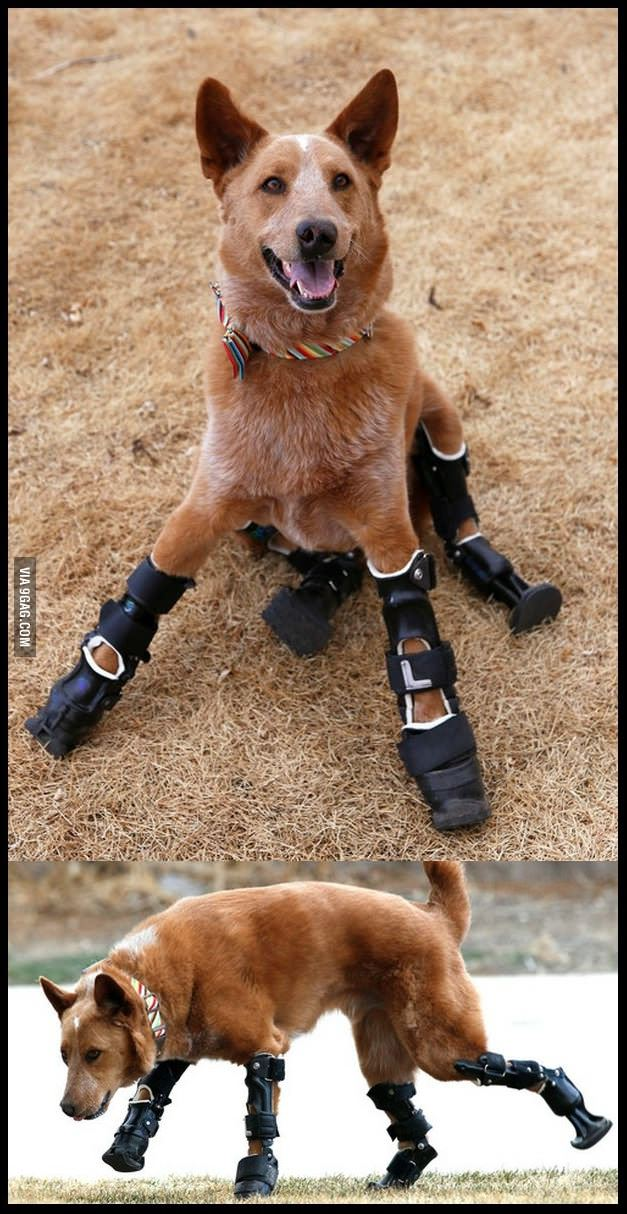
\includegraphics[width=0.8\textwidth]{graphics/dog.jpg}
					\label{graph:mems}	
					\caption{Przegląd technologi w ujęciu inwazyjności \cite{tenore}}
				\end{figure}
			\end{center}
		\end{frame}		
		
		\begin{frame}
			Prowadzone są badania nad trzema sposobami przesyłania informacji zwrotnej:
			\begin{itemize}[<+->]
				\item sprzężenie wibracyjne,
				\item sprzężenie elektryczne (pobudzanie skóry poprzez elektrody),
				\item sprzężenie bezpośrednio do nerwów:
				\begin{itemize}[<+->]
					\item przekazywanie informacji bezpośrednio do mózgu,
					\item przekazywanie informacji do nerwów w kikucie.
				\end{itemize}
			\end{itemize}
		\end{frame}
		
		\begin{frame}
		\begin{figure}
				\begin{center}
        			\begin{subfigure}[b]{0.5\textwidth}
                		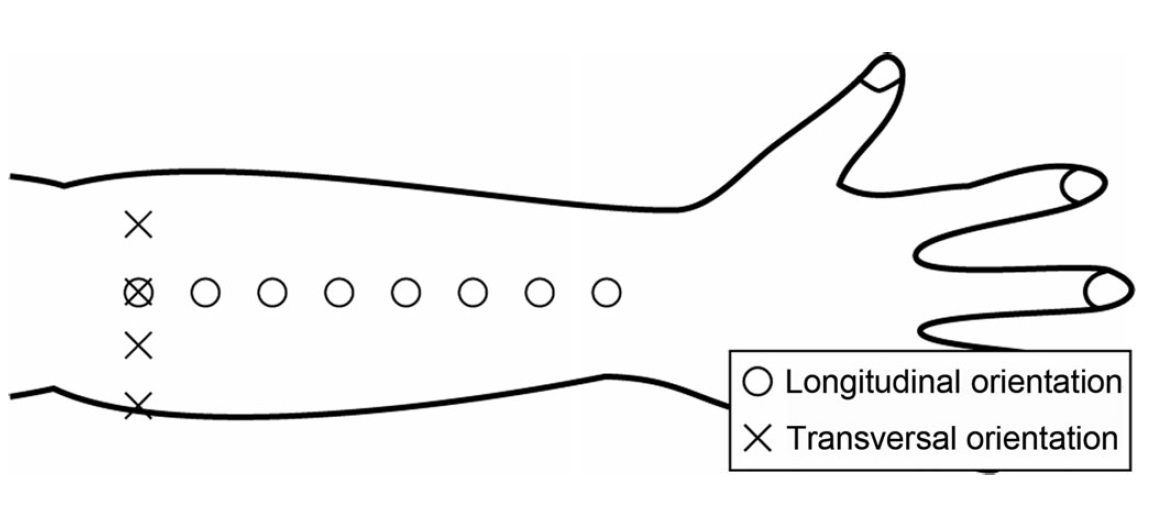
\includegraphics[width=\textwidth]{graphics/vibro_orientation.jpg}
                		\label{graph:g5}
        			\end{subfigure}%
        			\begin{subfigure}[b]{0.5\textwidth}
                		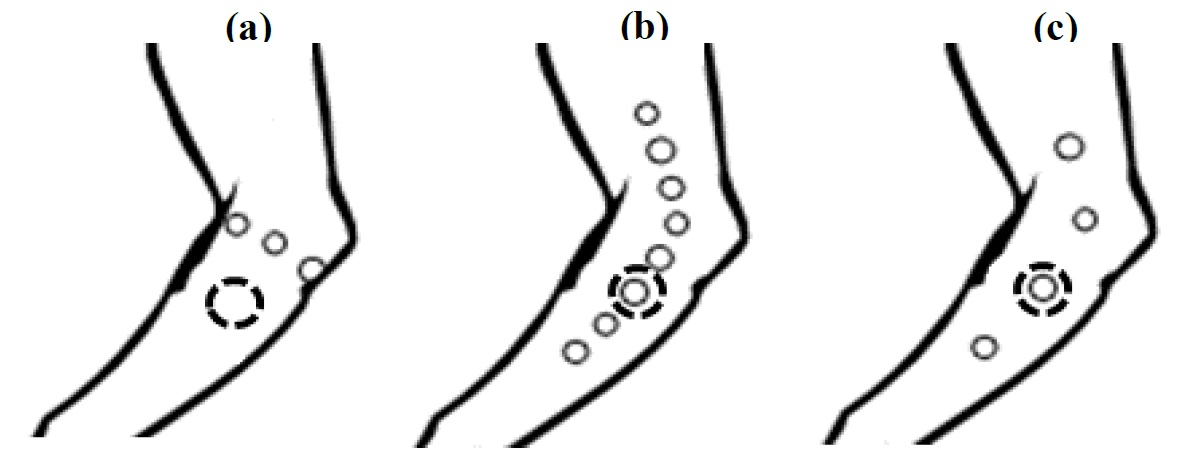
\includegraphics[width=\textwidth]{graphics/vibro_possib.jpg}
                		\label{graph:g6}
        			\end{subfigure}%
        			\newline
        			\begin{subfigure}[b]{0.7\textwidth}
                		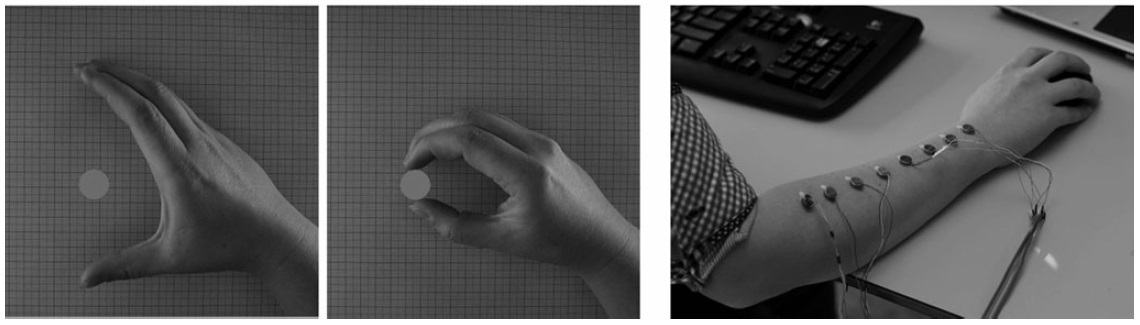
\includegraphics[width=\textwidth]{graphics/vibro_photo.jpg}
                		\label{graph:g6}
        			\end{subfigure}%
				\caption{Sprzężenie wibrostymulacyjne. \cite{tenore} }
				\end{center}
			\end{figure}
		\end{frame}
		
		\begin{frame}
		\begin{figure}
				\begin{center}
        			\begin{subfigure}[b]{0.6\textwidth}
                		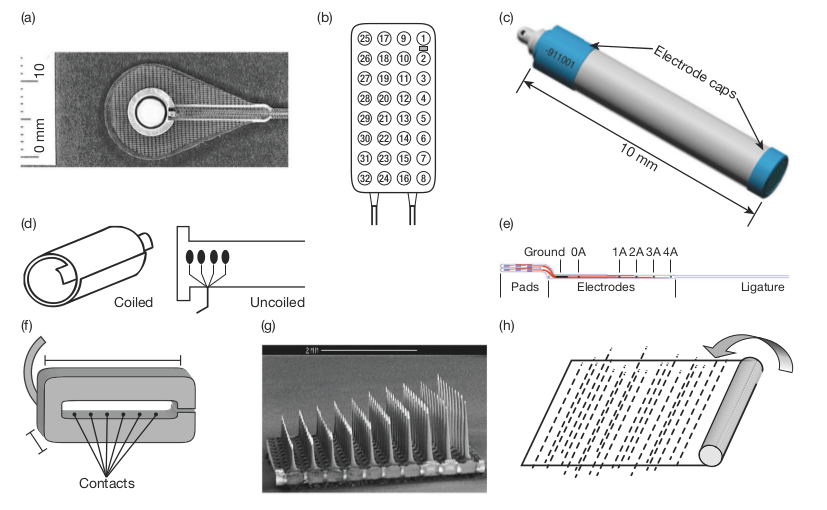
\includegraphics[width=\textwidth]{graphics/elektrode.png}
                		\label{graph:g5}
        			\end{subfigure}%
        			\begin{subfigure}[b]{0.4\textwidth}
                		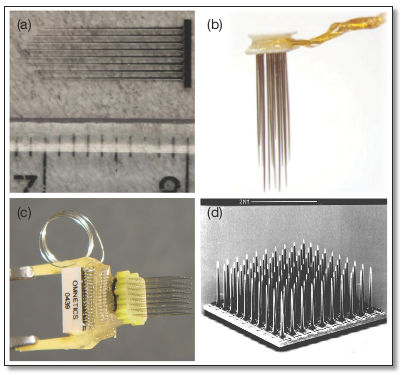
\includegraphics[width=\textwidth]{graphics/elektrode2.png}
                		\label{graph:g6}
        			\end{subfigure}%
				\caption{Mikroelektrody penetrujące. \cite{tenore} }
				\end{center}
			\end{figure}
		\end{frame}		
		
		
		
		\begin{frame}
			\begin{center}
				\begin{figure}
					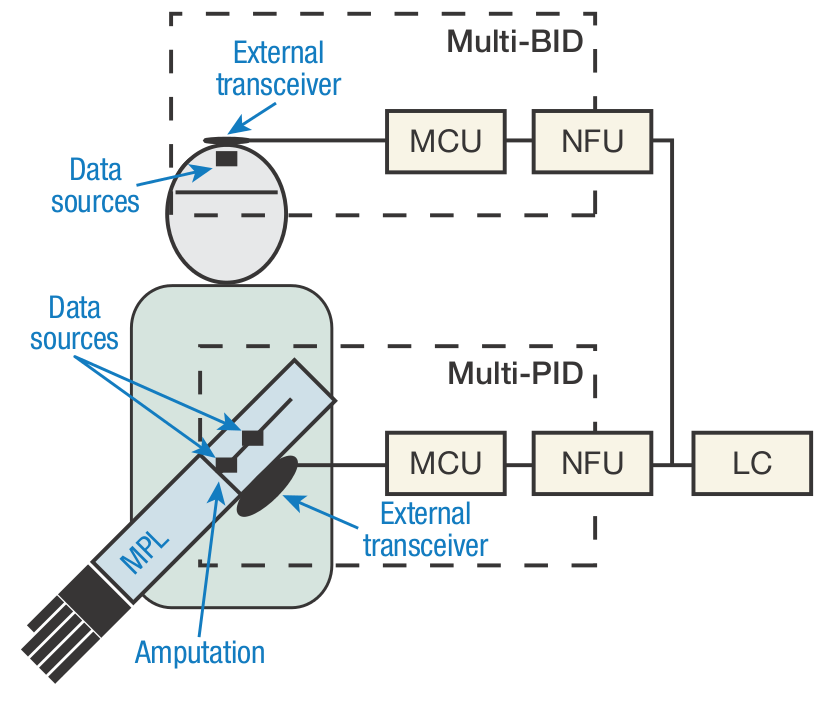
\includegraphics[width=0.7\textwidth]{graphics/MPL_ster.png}
					\label{graph:mems}	
					\caption{Sprzężenie zwrotne w protezie MPL \cite{tenore}}
				\end{figure}
			\end{center}
		\end{frame}	

	\subsection{Dostępne technologie}
		\begin{frame}
			\begin{center}
				\begin{figure}
					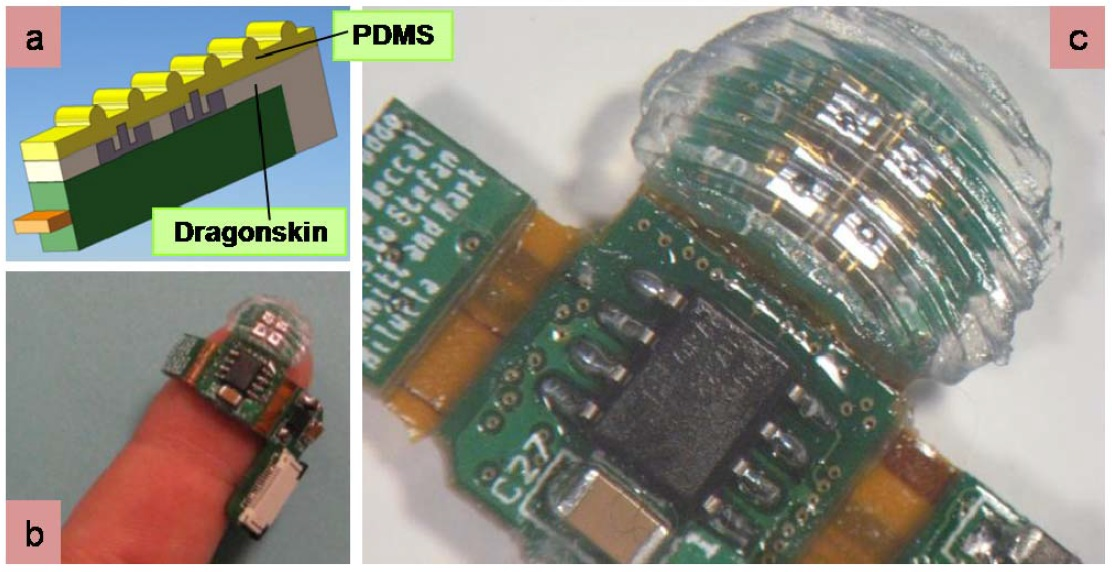
\includegraphics[width=\textwidth]{graphics/roughness_mems.jpg}
					\label{graph:mems}	
					\caption{ \cite{5420491}}
				\end{figure}
			\end{center}
		\end{frame}		
		
		
		\begin{frame}
		\begin{figure}
				\begin{center}
				
        			\begin{subfigure}[b]{0.4\textwidth}
                		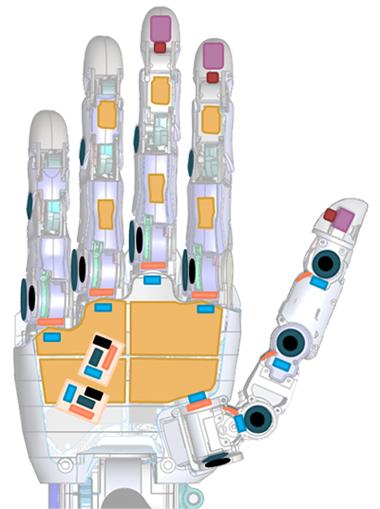
\includegraphics[width=\textwidth]{graphics/MPL_sensorhand.jpg}
                		\label{graph:g5}
        			\end{subfigure}%
        			\begin{subfigure}[b]{0.4\textwidth}
                		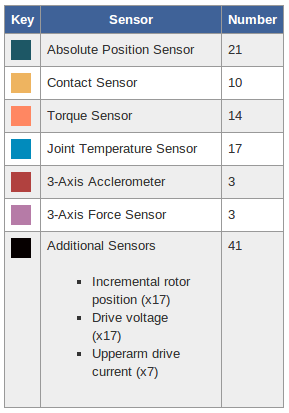
\includegraphics[width=\textwidth]{graphics/mpl_opis.png}
                		\label{graph:g6}
        			\end{subfigure}%
				\end{center}
				\caption{Sensory protezy MPL.}
			\end{figure}
		\end{frame}				
%
%		\begin{frame}
%		\begin{figure}
%				\centering
%                		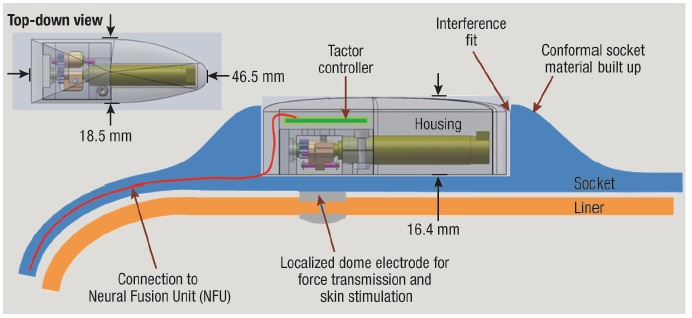
\includegraphics[width=0.7\textwidth]{graphics/vibro_mpl.jpg}
%				\caption{Wibrostymulacja dla protezy MPL.}
%			\end{figure}
%		\end{frame}	
	
		
	
\section{Propozycja rozwinięcia ręki BeBionic}
	
\begin{frame}[allowframebreaks]%{Propozycja rozwinięcia ręki BeBionic}
	Proponujemy zamianę karbonowej obudowy fabrycznej na obudowę zawierającą następujące czujniki:
	\begin{itemize}
		\item czujnik siły $\rightarrow$ FSR 400 Short
			\begin{figure}
				\begin{center}
        			\begin{subfigure}[b]{0.15\textwidth}
                		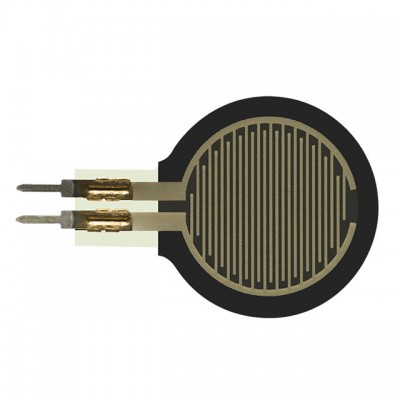
\includegraphics[width=\textwidth]{graphics/fsr400.jpg}
                		\label{graph:g5}
        			\end{subfigure}\hspace{2cm}
        			\begin{subfigure}[b]{0.3\textwidth}
                		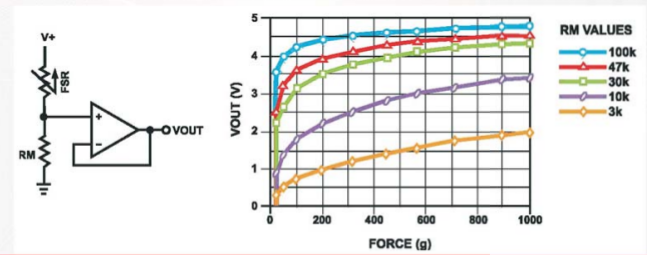
\includegraphics[width=\textwidth]{graphics/fsr400_app.png}
                		\label{graph:g6}
        			\end{subfigure}%
				\end{center}
			\end{figure}
	
			zalety: tanie, małe, proste w podłączeniu.
		\item czujnik prądu płynącego w silniku $\rightarrow$ ACS711
		\begin{figure}
				\begin{center}
        			\begin{subfigure}[b]{0.15\textwidth}
                		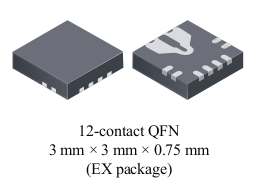
\includegraphics[width=\textwidth]{graphics/acs711.png}
                		\label{graph:g5}
        			\end{subfigure}\hspace{2cm}
        			\begin{subfigure}[b]{0.3\textwidth}
                		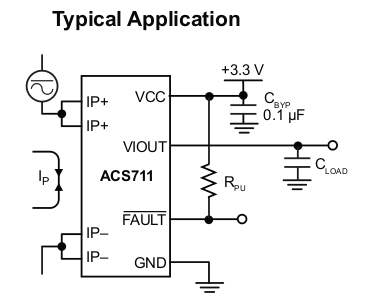
\includegraphics[width=\textwidth]{graphics/acs711_app.png}
                		\label{graph:g6}
        			\end{subfigure}%
				\end{center}
			\end{figure}
			
		
	\end{itemize}
\end{frame}

\begin{frame}
\begin{itemize}
\item akcelerometry na końcówki palców $\rightarrow$ ADXL362
			\begin{center}
				\begin{figure}
					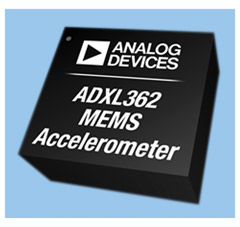
\includegraphics[width=0.2\textwidth]{graphics/adxl362.jpg}
				\end{figure}
			\end{center}
\end{itemize}
\end{frame}

\section*{Bibliografia}

\begin{frame}[allowframebreaks]
	\bibliography{bibliography}
\end{frame}
		
\begin{frame}
\begin{center}
				\begin{figure}
					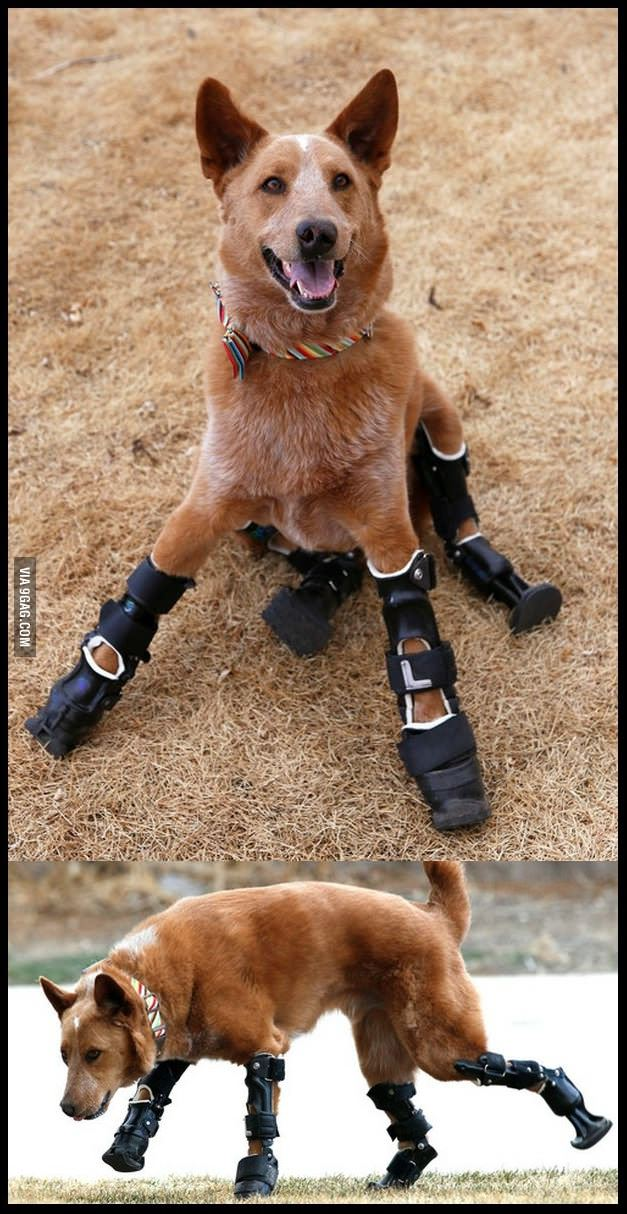
\includegraphics[width=0.3\textwidth]{graphics/dog.jpg}
					\caption{Naki’o now has 4 prosthetic legs and is able to run around happily!}
				\end{figure}
			\end{center}
\end{frame}

\end{document}
